\documentclass{fkssolpub}

\usepackage[czech]{babel}
\usepackage{fontspec}
\usepackage{fkssugar}
\usepackage{amsmath}
\usepackage{graphicx}

\author{Ondřej Sedláček}
\school{Gymnázium Oty Pavla} 
\series{2j}
\problem{2} 

\begin{document}

\begin{figure}[h!]
	\centering
	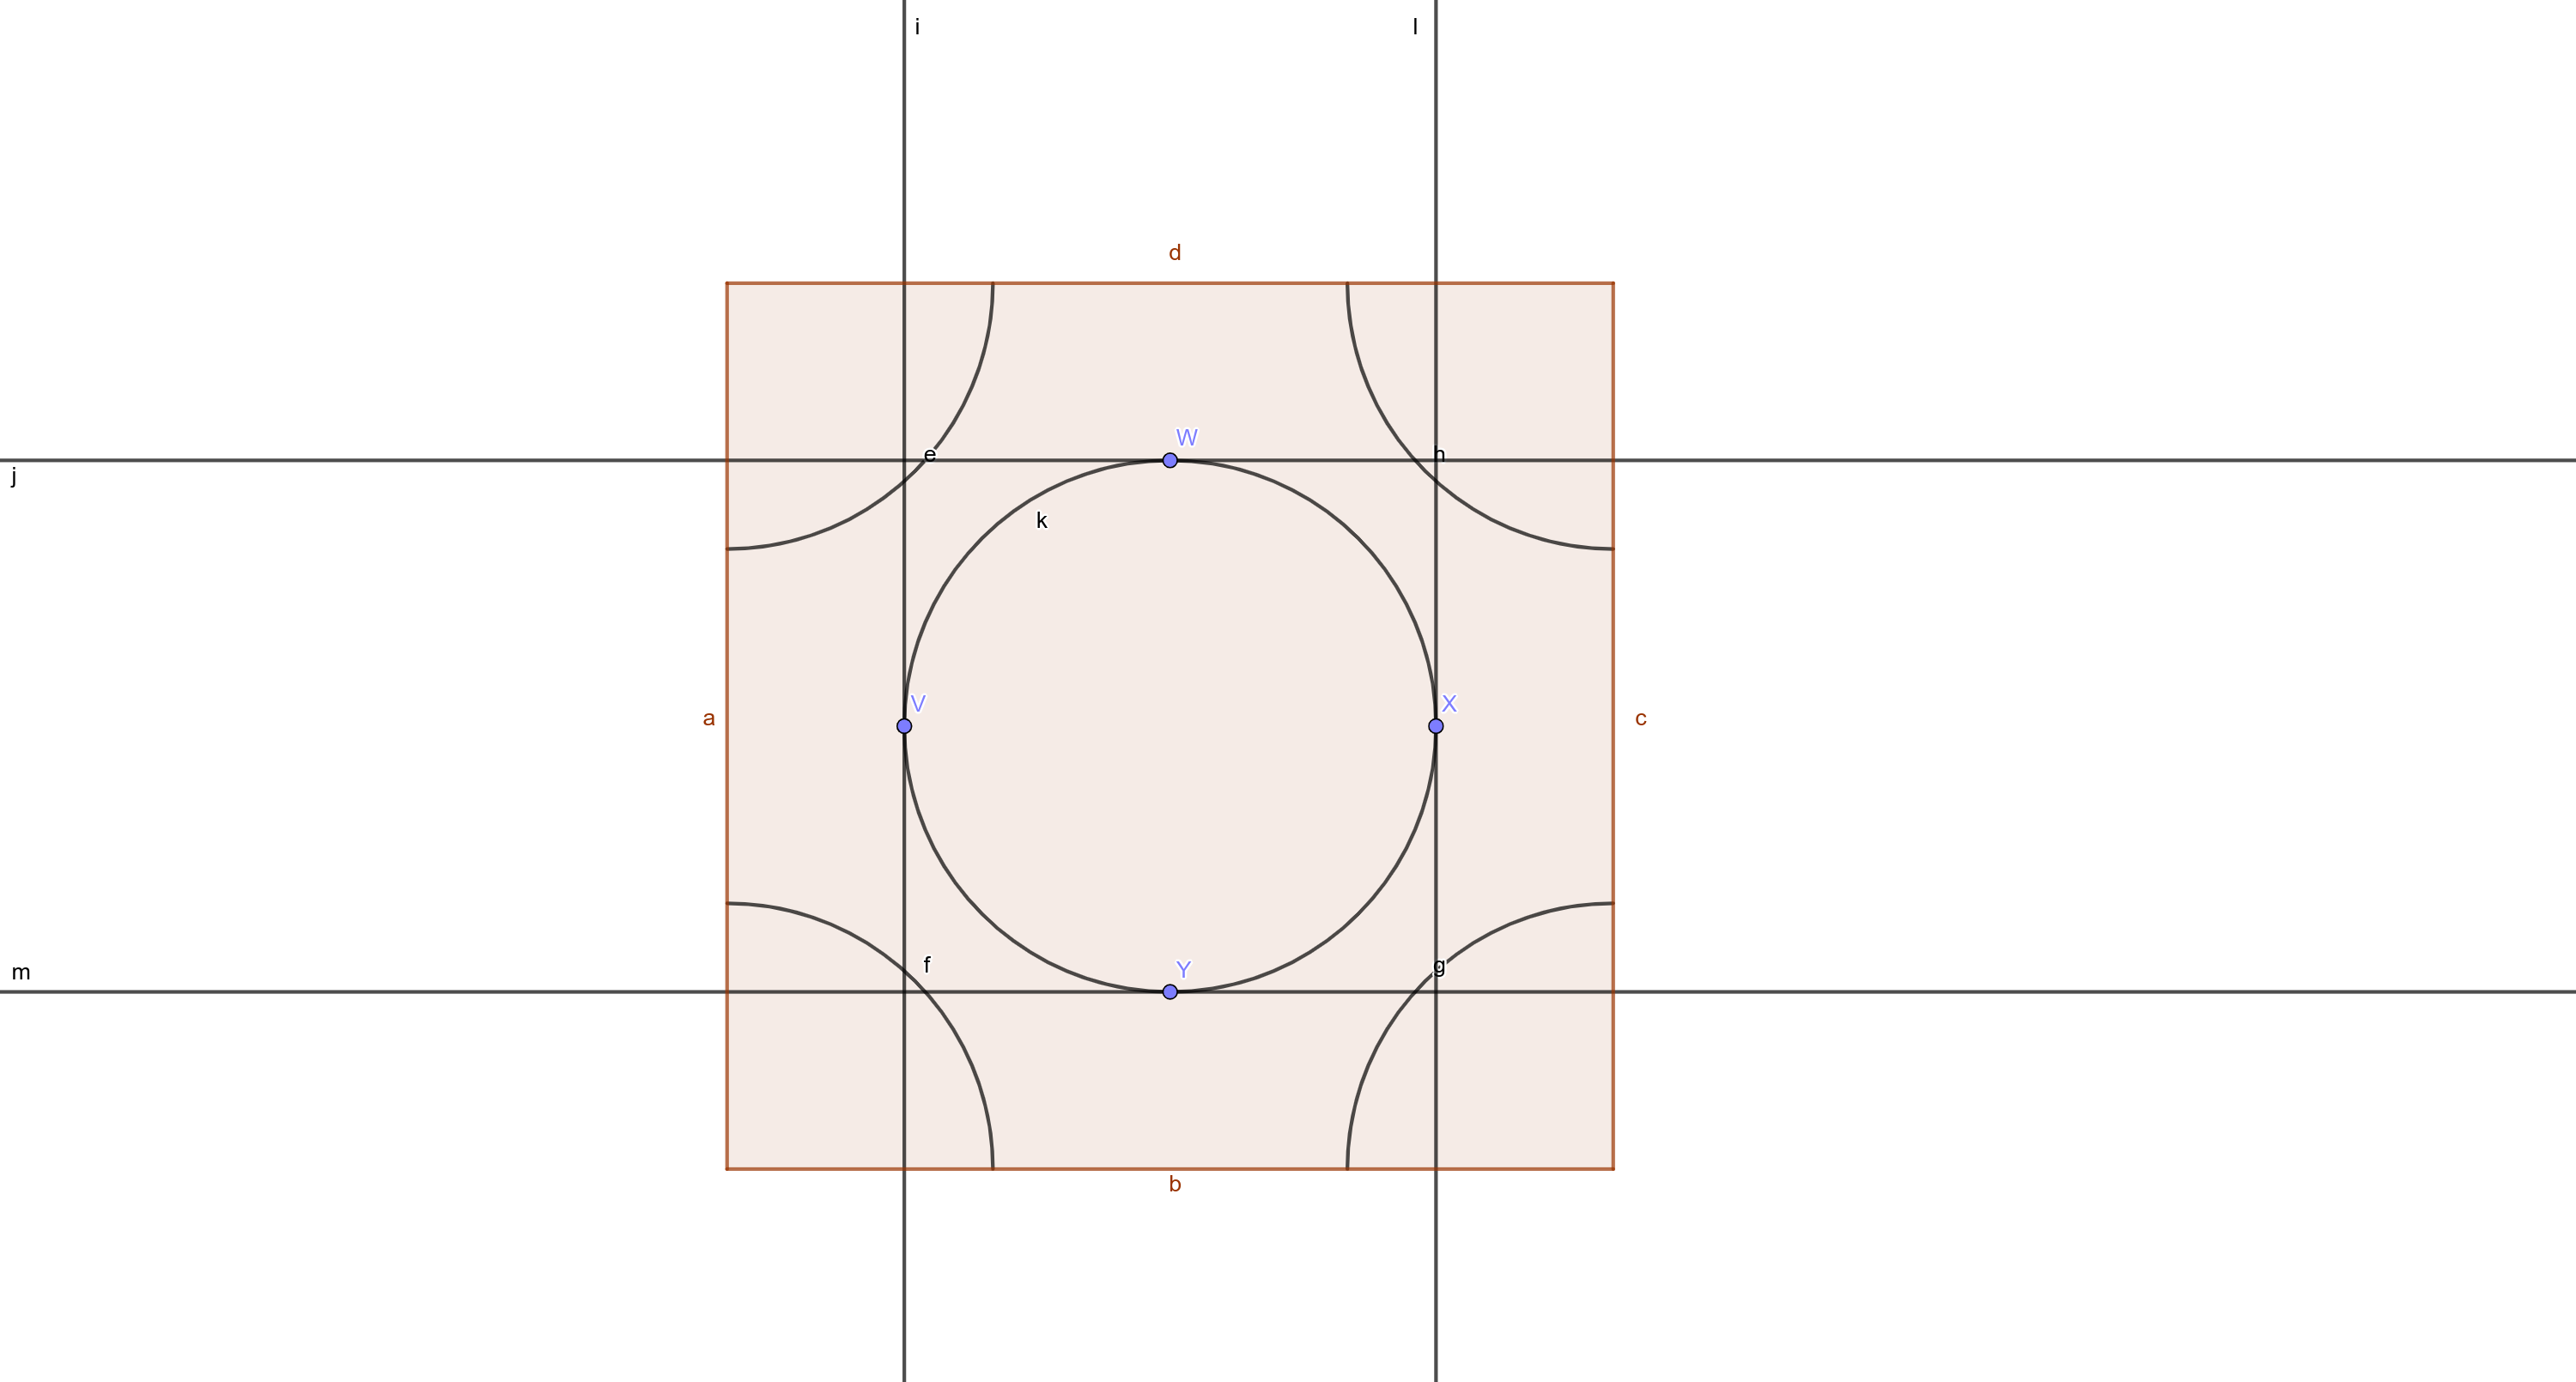
\includegraphics[width=0.95\textwidth]{2-fig.png}
	\caption{Rozmístění splňující zadání}
	\label{fig:sol}
\end{figure}

Rozmístění splňující zadání je takové, že body položíme na okraj kruhu tak,
jako jsou položeny body $V, W, X, Y$ na obrázku výše. Důvod, proč tohle rozmístění
splňuje zadání, je takový, že aby nějaký bod viděl alespoň dva body, musí ležet
v průnik polorovin určenými tečnami procházející kamarády. Tento průnik se ale
nachází v čtvrtkruhu v rohu, tudíž se tam pátý kamarád nemůže dostat. Tím pádem
toto rozmístění splňuje zadání.

\end{document}
